\chapter{Soccer Simulation 2D}\label{chapter:ss2d}
In this chapter we explain the architecture of the Simulator itself. It is divided in 5 sections: about RoboCup Soccer Simulation Server (rcssserver), \cite{rcssserver}, explanation of the formation tactics and the formation editor, a section about the two major agents: the coach and the players; and a Section to show the environment used to train our agents.

\section{Server}\label{section:rcssserver}
Robocup Soccer Simulation Server (RCSSS) is the core of SS2D. It processes the whole environment receiving the messages from every agent and returning the actual state of the game in discretized time. An old challenge to teams in the league is that the returned state is noisy, therefore, not fully trustful. Also, it establishes the communication between the communication with monitors, from which one can watch the game. 

RCSSS follows an UDP/IP client-server style, which allows teams to develop on any programming language since they do that communication. There's an specific port for the 11 infield players and another to the coach. Only messages with the allowed protocols is processed by the server. For example, only the goalie can do catch, if any other player do catch, the action is invalidated and the agent looses a cycle. The two agents with special commands are the goalie and the coach, which will be explained in Section \ref{section:coach}.  

After the initial connection with the clients, the server commits the it's parameters. Those parameters are divided in server-params, the environment itself (position of goal, size of ball, how many cycles it will wait for an action, etc), and the 18 player types. Each player type has random params for speed, acceleration, size (which influences in the tackle action), maximum stamina and kickable area. In game, clients can exchange N messages with other clients, N being given by the server-params.

\begin{figure}[H]
    \centering
    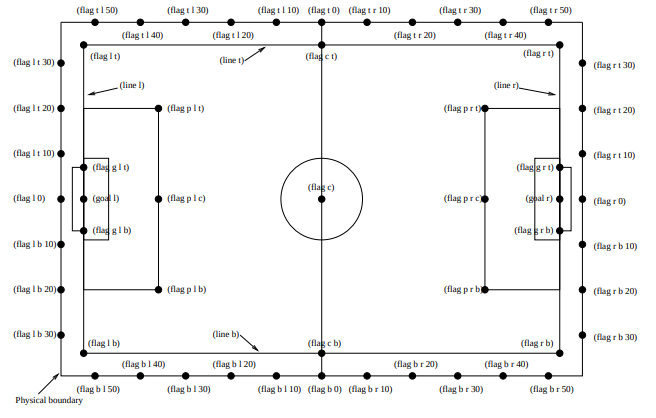
\includegraphics[scale=0.5]{images/field_params.png}
    \caption{Default field parameters given by the server. Image from \cite{ss2dmanual}.}
    \label{fig:fieldparams}
\end{figure}

\section{Formation}\label{section:formation}
The formation file is one of the most tactical information that the players have. It describes positions depending on ball's position and, for an agent based on Helios Base, also called Agent2D, (\cite{heliosbase}), like great part of the teams in the league, it is indispensable this information. With the Agent2D, it was also released Fedit2. It is an user interface(UI) that you can create formations files with up to 128 static situations. See Figure \ref{fig:fedit2}.

Teams usually have more than one formation file to be used in game. The formations can be changed given a certain situation. For example, if our team is winning and has great chance of winning, we can choose an aggressive formation instead of a defensive one.

\begin{figure}[H]
    \centering
    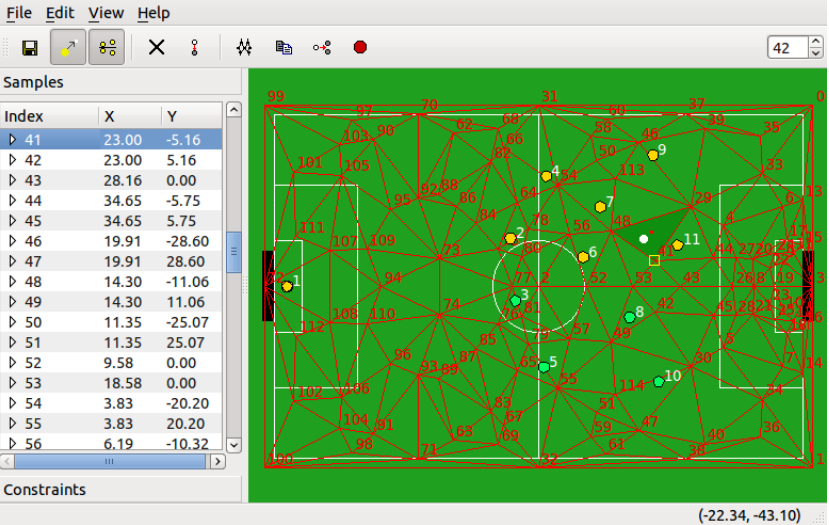
\includegraphics[scale=0.4]{images/fedit2.png}
    \caption{Actual Footage of Fedit2. Image from \cite{heliosbase}.}
    \label{fig:fedit2}
\end{figure}

\section{Agents}\label{section:agents}
In this section we shall talk about the main High-level agents: Coach and Player. The idea of each agent is based on a real soccer game where there is a coach and 11 players, where the coach can note things that the players cannot but they can send a message to a specific agent and only the player can execute the actions that the coach instructed them.

\subsection{Coach}\label{section:coach}
The coach is an special agent which can see all the field noiseless and has the greater message area of any agent. As it has global vision of the game, it can analyze globally the game (e.g: where our defense line is breaking, how we do goals more often, how many passes we got right). Cyrus2014, \cite{cyrus2014}, realized their code which shows some statistical information of the game. See Figure \ref{fig:cyrus_coach}.

For the next RoboCup, the teams will not be able to see each others names, so strategies developed for a given team will be more difficult to be applied. For that, the coach is the most quoted agent to analyse the game in real time and tell what probable team is the opponent and then apply the specific strategy.
\begin{figure}[H]
    \centering
    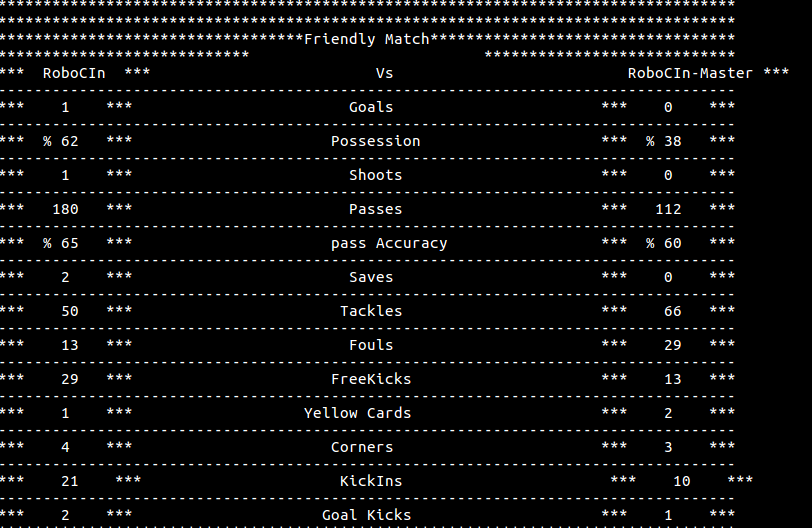
\includegraphics[scale=0.5]{images/cyrus_coach.png}
    \caption{Example of game analysis by Cyrus2014's coach.}
    \label{fig:cyrus_coach}
\end{figure}

\subsection{Players}\label{section:players}
The players are the usual agents in field. The players can take 8 actions:

\begin{itemize}
    \item Dash: given a power of dash $\alpha \in [-100, 100]$, the agent "runs" with $\alpha$ in its body's direction.
    \item Turn: given an angle $\gamma \in [-180, 180]$, the agent turns its body in $\gamma$ degrees.
    \item Kick: given a power $\alpha \in [-100, 100]$ and an angle $\gamma \in [-180, 180]$, the agent kicks in $\gamma$ direction with power $\alpha$.
    \item Tackle: given a power $\alpha \in [-100, 100]$, the agent tackles the ball.
    \item Say: given a message M and a target N, the agent sends to server M to delivered to N.
    \item Turn\_neck: given an angle $\gamma \in [-180, 180]$, the agent turns its neck in $\gamma$ degrees.
    \item Move: given a point (x,y) the agent is teletransported to (x,y). It is a special action done only while the game is paused.
    \item Catch: only the goalie can realize that action.
\end{itemize}
The agent has some restrictions of view as well. As far as the agent is of a target P, it becomes more difficult to see P. Figure \ref{fig:view_ranges} describes the view model, where point a, c and d the agent can see all parameters of P, at point e it cannot see the uniform number of P, at point f it cannot see which team P belongs to, at point b and g the agent cannot see. To cure some tactics that depends of all agents in field, \cite{heliosbase} created a memory for the agent that allows check an old position of the target. The catch and kick action also has some restrictions, it can only be performed if the ball is the kickable or catchable area. Figure \ref{fig:catchable_area} shows an example of catchable area.
\begin{figure}[H]
    \centering
    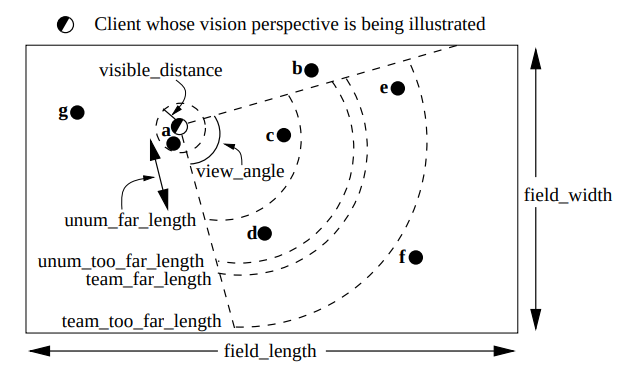
\includegraphics[scale=0.5]{images/view_ranges.png}
    \caption{Ranges of view of the players. Image from \cite{ss2dmanual}.}
    \label{fig:view_ranges}
\end{figure}

\begin{figure}[H]
    \centering
    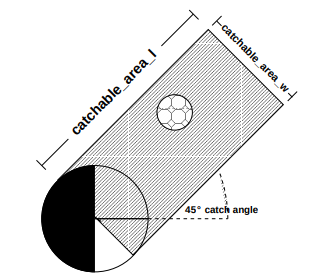
\includegraphics[scale=0.5]{images/catchable_area.png}
    \caption{Description of Catchable Area. Image from \cite{ss2dmanual}.}
    \label{fig:catchable_area}
\end{figure}


\section{Half Field Offensive}\label{section:HFO}
The Half Field Offensive (HFO), \cite{hfo}, is an interface environment designed specifically to train SARSA (state, action, reward, next state, next action) agents based on the usual OpenAI environments. HFO supports: a delayed message from the agent due to an algorithm training or some heavy process, writing the agent's code in Python Programming Language (\cite{python}) using the original actions of the C++ Programming Language (\cite{cpp}) agent via an interface, see figure \ref{fig:HFO_diagram}. It provides 2 spaces of states and actions:
\begin{itemize}
    \item Low-Level Features and Actions- Uses raw features from SS2D server (angle, positioning) and provides raw actions (kick, dash, turn).
    \item High-Level Features and Actions - Uses processed features (distance to opponent, interceptable ball) and only complex or chained actions (dribble, pass to teammate).
\end{itemize}

\begin{figure}[H]
    \centering
    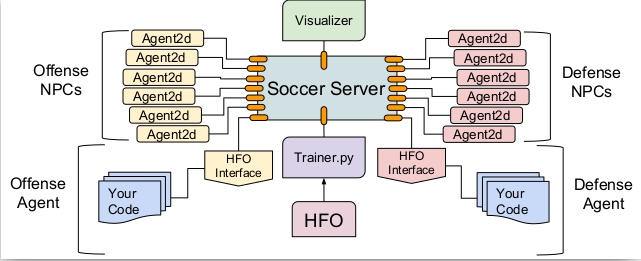
\includegraphics[scale=0.5]{images/HFO_diagram.png}
    \caption{Half Field Offensive diagram. Image from \cite{hfo}.}
    \label{fig:HFO_diagram}
\end{figure}